\section{UFO: a non-alien ontology} 

If the objective is to engineer an ontology there are many ways to take on this challenge. When the ontology to be engineered is of the domain or task type, a top-level, or more commonly named, foundational ontology is needed as basis for the new model. Altogether, an application ontology needs both a domain and a task ontology as a basis. How to address the creation of a top-level ontology is a complicated work and not on the scope of this text. It suffices to say that they are needed to build the other ontologies. In other words, domains and tasks are modeled using a foundational ontology and aplications are modeled combining a domain ontology and a task ontology.

Before delving deeper in UFO modeling specifications and concepts it is important to expose the perspective it uses to model the world. First it is necessary to understand what are endurant and perdurant. Such concepts are introduced and studied in philosophy. They divide the being, or that which exists, in two possibilities, either it is a endurant or a perdurant. The former is a being that exists in time, it can be analyzed independently of the time. The latter is a beign which happens over time, and it needs that time-span to exists, thus is not independent of it. In a more simplistic manner one can say that perdurant are events and endurants are everything else. 

UFO or Universal Foundational Ontology created by \cite{guizzardi_ontological_2005}, is one of the most complete and used foundational ontologies in computer sciences. It leans on a heavy philosophical background and precise logical structure to provide a most complete modeling language. It is divided into different specifications UFO-a for endurants and UFO-b for perdurants. This work utilizes UFO-a because it is an ontology of an endurant and does not use UFO-b specifications. As such this section focus on UFO-a only. For simplicity whenever it is written UFO it is addressing UFO-a only.

\subsection{The Universal}

Central concept of the UFO is that of an \textit{universal}, it is the common proprieties found in different individuals. The concept is akin to a class or type in many of the modeling languages. It provides the common characteristics of a group of individuals. 

There are diverse types of universals which are classified according to how they deliver meaning to an individual. The first classification to be remarked is the distinction between sortal and dispersive. `` ... a Sortal Universal, which provides a \textit{principle of individuation} and \textit{identity} to the particulars it collects'' \citep{guizzardi_ontological_2005}. A dispersive universal embrace many concepts with different identities and thus do not convey a principle of individuation for its instances.

Sortal is a term coined by John Locke in \cite{locke1841essay}. A technical philosophical term which was further developed by other authors. This notion is central to the discussion of things. A sortal has three main characteristics according to \cite{sep-sortals}:

\begin{itemize}
    \item Tells us what the essence of a thing is
    \item Tells us how to count things of that kind, which requires knowing which things are different and which are the same
    \item Tells us when something continues to exist, and when it goes out of existence
\end{itemize}

Thus a sortal is what individualizes different things and specifies. Allowing us to discuss about those things accounting for all its proprieties. It answers the question of ``What is it?''.

Rigidity of an universal provides another differentiation quality. ``A rigid universal is one that applies to its instances necessarily, i.e. in every possible world"\citep{guizzardi_ontological_2005}. For example, if there is a universal for \textit{Man} which specifies \textit{Person} in any possible world a given real person is identified by the person concept. While if it is a man it provides further identification, it is not a woman, and it remains a man in every possible world. An universal can also be \textit{non-rigid} which is the logical negation of rigid or \textit{anti-rigid} which is a more constraint form of non-rigid.

A universal which does not apply necessarily to at least one of its instances is non-rigid. \textit{Seatable} provides a nice example, suppose its instances are a given chair and a crate. The chair is necessarily seatable in every world whilst the crate can become unsteable and still be the same crate. Anti-rigid restricts that for every instance of the universal it must exist a world where it does not apply to that instance. Following the person example, a given man could be specified by the universal \textit{Child}, but it is only a child in his early years of life, in all other worlds he is no longer a child but an adult or elder.

Upon this classification \citeauthor{guizzardi_ontological_2005} brought together a typology for universals. This typology classifies and names the types of possible universals in UFO. This structure is depicted in \autoref{fig:Univ_diag}. Each of its leaves is a final classification for universals which are very important concepts for conceptual modeling. Those are defined and explained in the remainder of this section.

%Universal diagram
\begin{figure}[ht!]
\centering
\scalebox{0.65}{
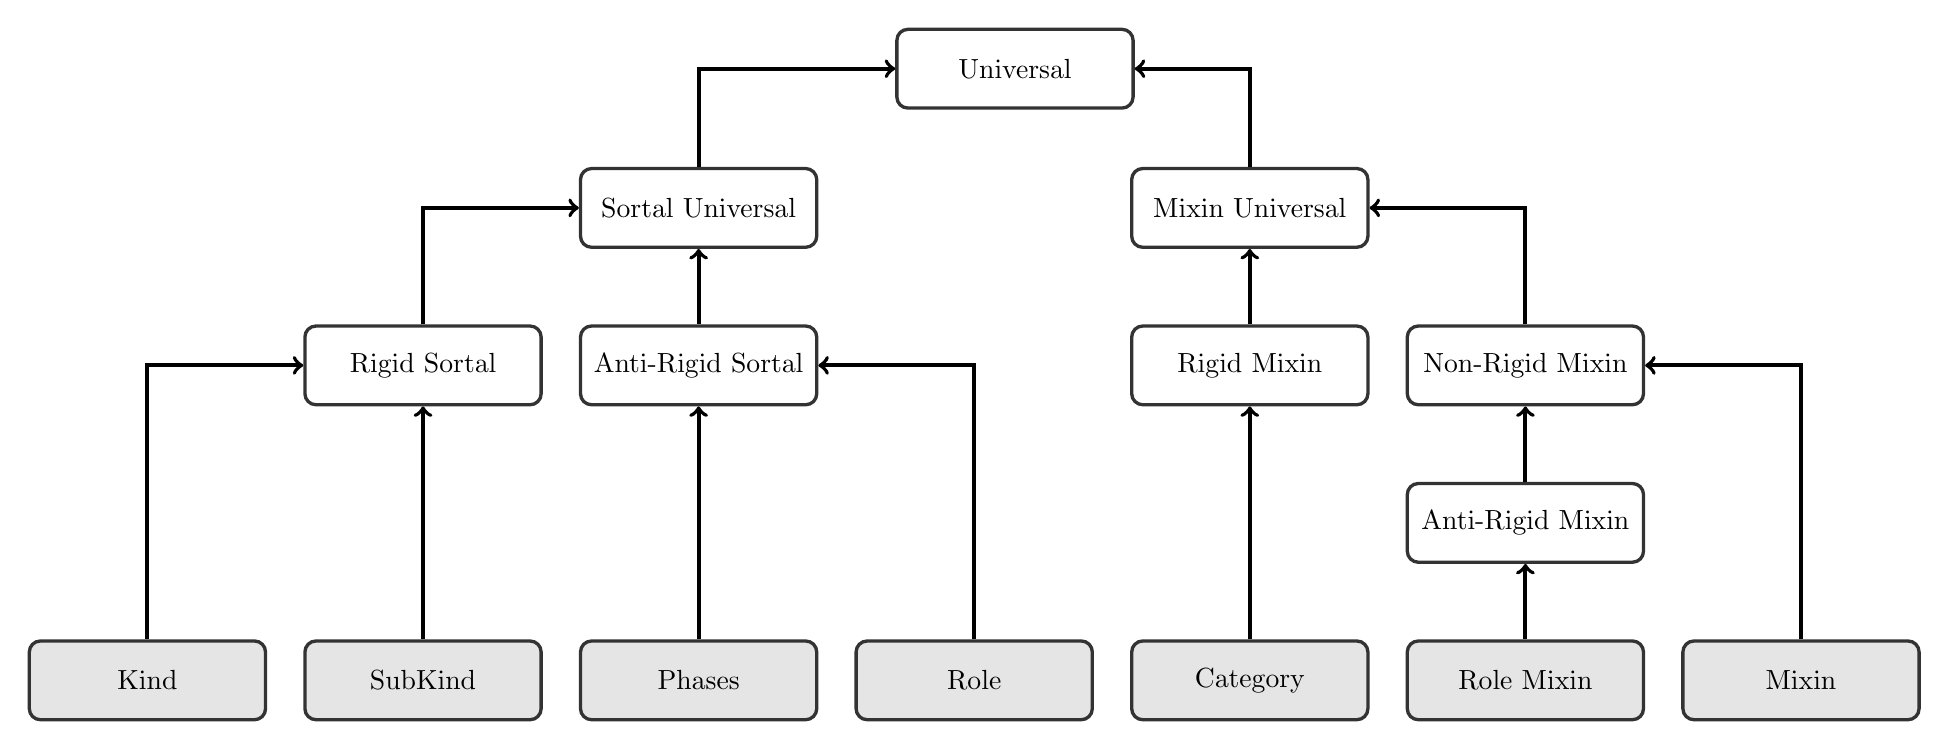
\begin{tikzpicture}[squarednode/.style={rectangle, 
					rounded corners, 
					very thick,
 					minimum width=3cm,
					minimum height=1cm,
					draw=black!80, 
					fill=white!10},
					squarednode2/.style={rectangle, 
					rounded corners, 
					very thick,
 					minimum width=3cm,
					minimum height=1cm,
					draw=black!80, 
					fill=black!10},
					node distance = 2.5cm
					]
					


%top node
\node[squarednode]  (Univ) {Universal};

%second level
\node[squarednode]  (Sortal) [below left of = Univ, xshift=-2.25cm] {Sortal Universal};
\node[squarednode]  (Mixin) [right of = Sortal, node distance = 7cm] {Mixin Universal};

% third level
\node[squarednode]  (ARigidSor) [below of = Sortal, node distance = 2cm] {Anti-Rigid Sortal};
\node[squarednode]  (RigidSor) [left of = ARigidSor, node distance = 3.5cm] {Rigid Sortal};

\node[squarednode]  (RigidMix) [below of = Mixin, node distance = 2cm] {Rigid Mixin};
\node[squarednode]  (NRigidMix) [right of = RigidMix, node distance = 3.5cm] {Non-Rigid Mixin};
\node[squarednode]  (ARigidMix) [below of = NRigidMix, node distance = 2cm] {Anti-Rigid Mixin};

% leaves
\node[squarednode2]  (SubKind) [below of = RigidSor, node distance = 4cm] {SubKind};
\node[squarednode2]  (Kind) [left of= SubKind, node distance = 3.5cm] {Kind};


\node[squarednode2]  (RoleMix) [below of = ARigidMix, node distance = 2cm] {Role Mixin};
\node[squarednode2]  (MixinL) [right of= RoleMix, node distance = 3.5cm] {Mixin};

\node[squarednode2]  (Cat) [below of = RigidMix, node distance = 4cm] {Category};

\node[squarednode2]  (Phases) [below of = ARigidSor, node distance = 4cm] {Phases};
\node[squarednode2]  (Role) [right of=Phases, node distance = 3.5cm] {Role};



% Arrows 
\draw [->, line width=0.5mm] (Sortal.north) |- (Univ.west);
\draw [->, line width=0.5mm] (Mixin.north) |- (Univ.east);

\draw [->, line width=0.5mm] (RigidSor.north) |- (Sortal.west);
\draw [->, line width=0.5mm] (ARigidSor.north) -- (Sortal.south);
\draw [->, line width=0.5mm] (NRigidMix.north) |- (Mixin.east);
\draw [->, line width=0.5mm] (RigidMix.north) -- (Mixin.south);
\draw [->, line width=0.5mm] (ARigidMix.north) -- (NRigidMix.south);

\draw [->, line width=0.5mm] (Kind.north) |- (RigidSor.west);
\draw [->, line width=0.5mm] (SubKind.north) -- (RigidSor.south);
\draw [->, line width=0.5mm] (Phases.north) -- (ARigidSor.south);
\draw [->, line width=0.5mm] (Role.north) |- (ARigidSor.east);
\draw [->, line width=0.5mm] (Cat.north) -- (RigidMix.south);
\draw [->, line width=0.5mm] (RoleMix.north) -- (ARigidMix.south);
\draw [->, line width=0.5mm] (MixinL.north) |- (NRigidMix.east);

\end{tikzpicture}
}%endscale
\caption{Universal classification Diagram}
\label{fig:Univ_diag}
\end{figure}

Gray nodes at the bottom of the diagram are the types of universals present in UFO. Each contains the fundamental characteristics that define the concepts of the model. The arrows forms the specification path from which that type comes. Kind is a rigid sortal, which is a sortal universal that is a universal, and so on. Whatsoever each leave has its own meaning and definition that allows the modeler to stereotype each concept representing a universal.

``<<kind>> represents a \textit{substance sortal} that \textit{supplies} a principle of identity for its instances'' \citep{guizzardi_ontological_2005}. The kind is then the representation of what is a rigid sortal, that is, in a given model all concepts which are rigid sortals are kinds. Subkinds are just specializations of kinds and can be omitted from a model without any lost. Any object in a UFO specification must be an instance of a kind, directly or indirectly.

Phases are a specification of kinds, and represent the different states that a kind has along the time of its existence. It is important that, when modeled, the phases of a kind constitute all of the phases it has in the world. That is, when modeling a person, and including his \textit{adult} and \textit{elder} phases, it would be incorrect without a \textit{child} phase. Phases then form a partition of a given kind existence.

Roles determine how a given entity plays a role in a certain context. Differently from phases, which depends solely on intrinsic proprieties, roles depends on external proprieties, that is, how the entity relates to the other entities. Roles, then, need to be connected by a relationship to a external  kind. Using the person example, the kind person can be related to roles such as \textit{student}, but it does need to have a relationship, say \textit{enrollment}, with a \textit{school} kind. 

Mixin universals represents the dispersive concepts discussed before. Category is a collection of kinds, it is an abstract entity which unite common characteristics of the kinds it generalizes. Same is valid for Role Mixin, it is an abstraction of proprieties common to multiple Roles. 

The type defined as Mixin is basically everything else, it comprehends all non-rigid dispersive universals. Whatever fails to have the characteristics of the other types is a mixin. They represent properties which are essential to some instances but happens accidentally to the other ones. The best example to illustrate it is the seatable examples used previously, which it is essential to the chair but accidental to the crate.

Those classifications have a complete logical formal definition. Their description can be found in \cite{guizzardi_ontological_2005}.

\subsection{The wholes with parts}

Mereology is a very important component of ontologies. It is the theory which relates of the parts that compose a whole and how those parts relate to the whole. Simple as it may seem it is a very useful tool for accurately modeling complex wholes.

Defining parts and wholes in a very simple way may seem easy. Wholes are any concepts which has one or more parts and the concepts that together make up another one are parts. But this is not quite true for UFO, as it presents a \textit{principle of unity} in its mereology. For this principle to hold the parts of a whole need to be related between themselves, not only to the whole. Another diferentiation of this mereology is the existance of \textit{secondary characteristics of parts}. This defines the role a part play within the aggregate it belongs, i.e whether objects can share parts, or if an object can only exists if an specific part exists. 

Following is a further explanations of those important notions pertaining the theory of parts and wholes of UFO.

\subsubsection{Principle of unity}

Prime reason for this principle is to deal with a conceptual problem very common in many mereologies. That using this theories purely can lead to very weird compositions which are not cognitively acceptable. Think of a set of parts and two wholes composed by these same set of parts. Most simple theories state that these wholes are identical, which is not necessarily true. It is easy to think of a band as a whole composed of its musicians but they can also be part of a group of friends or even a family. 

Integral wholes is the name given to a set of parts that have this principle. In other words, that have a unifying condition which bonds them in a specific way. Such connection should be not only a simple relation of any kind, it needs to tie the parts together in a way that changes their history. A good example is given by a molecule of a mass of water that is $H_2O$. While it is composed of H and O atoms if they didn't had a molecular bonding between them, the sharing of electrons, they wouldn't be a molecule of water.

\subsubsection{Secondary characteristics}

Parts convey a lot of meaning to its wholes, and the secondary characterization focus on explicitly understanding and classifying this meaning. There are two types of roles for parts, intimately related to how they behave in respect to the whole. If a part can be shared by multiple wholes, it is a characteristic named \textit{shareability}, or if it is separable from its whole, name it \textit{separability}.

Terming them secondary is done to emphasize that not all relationships of this type has this propriety. That is, a part-hood relationship might not feature such characteristics, but when they do, it express more meaning into the conceptual relationship.

\subsubsection{Shareability}

Sheareability defines characteristics which address if a given part can be shared between different wholes. That is, if something can be a part of two different entities at the same time. With this it suffices to define a single type of part. 

The exclusive part, is a part-whole relationship that states that its a part of its related individual or its a part of something else that is by itself a part of the related individual or the opposite, it is part of something of which the related individual is also a part. In other words if a given engine is a exclusive part of a car, it can be a part of the chassis which is part of that car, but never part of a museum which is not a whole with the car as a part. It might seem confusing but the exclusive is a good name, and its meaning is well applied in this concept.

This concept can be extended from individuals to universals creating the general exclusive part-whole relationship. Is the same idea but relating universals instead of individuals, an universal A is a general exclusive part of an universal B, if every instance of A is exclusive part of some instance of B.

\subsubsection{Separability}

Understanding separability requires first to learn about ontological dependence. Existential dependence comes in a very intuitive way. If x is an individual existentially dependent of y, than necessarily y exists whenever x exists. Which can also be extended to universals creating the generic dependence. Individual z is generic dependant of the universal A, if whenever z exists some instance of A must exists.

Simply using the concept of dependence leads to a very intuitive secondary characteristic. Whenever there is a individual x and another one y, if y is existentially dependent of x and x is necessarily a part of y we say that x is an essential part of y. It is simply a part that without there is no whole, a good example is that one cannot have a living person without a brain, so brain is a essential part of living person. 

With this comes a notion of the extensional individual. It is the individual of which all of its parts are essential. That is, it needs all of its parts to exists, it cannot have some of them, it needs all of them.

Using the other side of existentially dependence one can introduce the concept of inseparable part. This is a part which is existentially dependent of its whole. Important distinction comes from this notion, an essential part is not necessarily a inseparable part. When inseparable a part lifespan of existence is completely tied to the whole that contains it. Whilst the essential part can exists without the whole. I.e, a chassis is an essential part of a car, but the chassis exists a long time before the car does, while a brain is an inseparable part of a living person it existence is tied to the lifespan of the living person.

Lastly the concept of inseparable part can be generalized using the generic dependence of the part to a whole. We say that a mandatory whole is the individual instantiating an universal from which the part is generic dependent. An example is the heart of a living person, it can exist before a specific person, but it needs a person to exists. It can change the instance of person it is part of through a transplant, but some person is mandatory for its existence.

\subsection{Restrictions}

Restrictions are the name of some logical rules that binds the ontology. Their importance comes from expressing some imitating concepts from the world within the modeling language.  \cite{guizzardi_ontological_2005} does not address this feature in his theoretical basis. Nonetheless it is necessary for the development of ontologies and is included in OntoUML specification, where it is presented in OCL scripting. \citep{guizzardi_ontoUML_2004}

Logical sentences form those rules. They bind the cardinality of certain relationships, the possibilities of generalization or even invalidate specific connections between some concepts. Restrictions like these have the purpose of impeding absurd representations of the modeled reality. In example, if in a model of persons we have an specification of man, an adult man, and it has a variable age. Without restrictions one could model an adult man with 10 years of age, which is an absurd. To correct this would be to add a restriction that for the adult man his age should be within 21 to 60 years.

Bureaucratic as they seem, restrictionships are essential to model ontologies. They provide means to express some limitations which can be hard to convey using the other ontological methods. Providing a way to introduce a logical reasoning inside the conceptual model, the rules, become a tool for the modeler to state how that reality works and behave. For the matter, in a given model it is possible to have a greater appropriateness using rules. That is, increasing the specificity of the model being able to be use abstraction about the reality intended.